\section{Results}
\label{sec:results}

In this section, we show results that support our initial conjecture that OCI convergence accelerates, more than SI, in transient transport calculations with decreased time step sizes.
We also further analyze OCI's performance on AMD MI250X GPUs using batched LAPACK solvers on a highly scattering problem from literature at multiple time step sizes and cell width values.

\subsection{Fourier analysis: transient iterative convergence rate}
\label{sec:results-faoci}

To study the impact of transient conditions on OCI we solve the Fourier system for steady-state and time-dependent transport derived in Section~\ref{sec:methods-faoci} both for simple corner balance in space.
For all Fourier analyses we sample $\lambda \in [0,2\pi]$ at \num{250} points and use \texttt{numpy.max(numpy.abs(numpy.eig(}$T$\texttt{)))} to compute spectral radius at a given point in parameter space ($\delta$ ($\Sigma\Delta x$), $\tau$ ($\Sigma v\Delta t$), and $c$ ($\Sigma_s$/$\Sigma$)) in S$_{8}$ using Gauss--Legendre quadrature.

Table \ref{table:difflimit} shows spectral radii produced from steady-state and transient OCI systems with various choices of mean free time ($\tau$), at various cellular optical thicknesses ($\delta$).
Steady-state predictions show the expected and previously published results that $\rho=1$ when $c=1$ regardless of $\delta$.
However, for the time-dependent system, $\rho<1$ regardless of the considered $\tau$ and $\delta$.
Furthermore, as $\tau$ shrinks and $\delta$ grows, $\rho$ dramatically decreases, approaching zero at the smallest $\tau$ and largest $\delta$.

\begin{table}[htb]
  \centering
  \begin{tabular}{@{}l c c c @{}} \toprule
    $\tau$ & $\delta=10.$ & $\delta=1.0$ & $\delta=0.1$ \\ \midrule
    SS  & \num{1.0000} & \num{1.0000} & \num{1.0000} \\
    10 & \num{0.99522} & \num{0.99952} & \num{0.99995} \\
    1  & \num{0.95323} & \num{0.99522} & \num{0.99952} \\
    0.1   & \num{0.64031} & \num{0.95321} & \num{0.99522} \\
    0.01 & \num{0.11177} & \num{0.63343} & \num{0.95351} \\
    \bottomrule
  \end{tabular}
  \caption{OCI spectral radius $\rho$ in the diffusive limit ($c=\Sigma_s/\Sigma =1.0$) from Fourier analysis at various mean free time ($\tau$) and cellular optical thickness ($\delta$) values. SS indicates steady state.} 
  \label{table:difflimit} 
\end{table}

Figure~\ref{fig:specrad_fa} shows $\rho$ predictions for OCI and SI produced from the Fourier system.
As previously published: as $\delta$ gets smaller, $\rho$ approaches 1 regardless of the scattering ratio.
As postulated in this work: as $\Delta t$ gets smaller, $\rho$ tends to 0---due to improvements in scattering ratio (which also affects SI) and increasing $\delta$---increasing the diagonal dominance of the iteration matrix.

\begin{figure}[htbp]
    \centering
    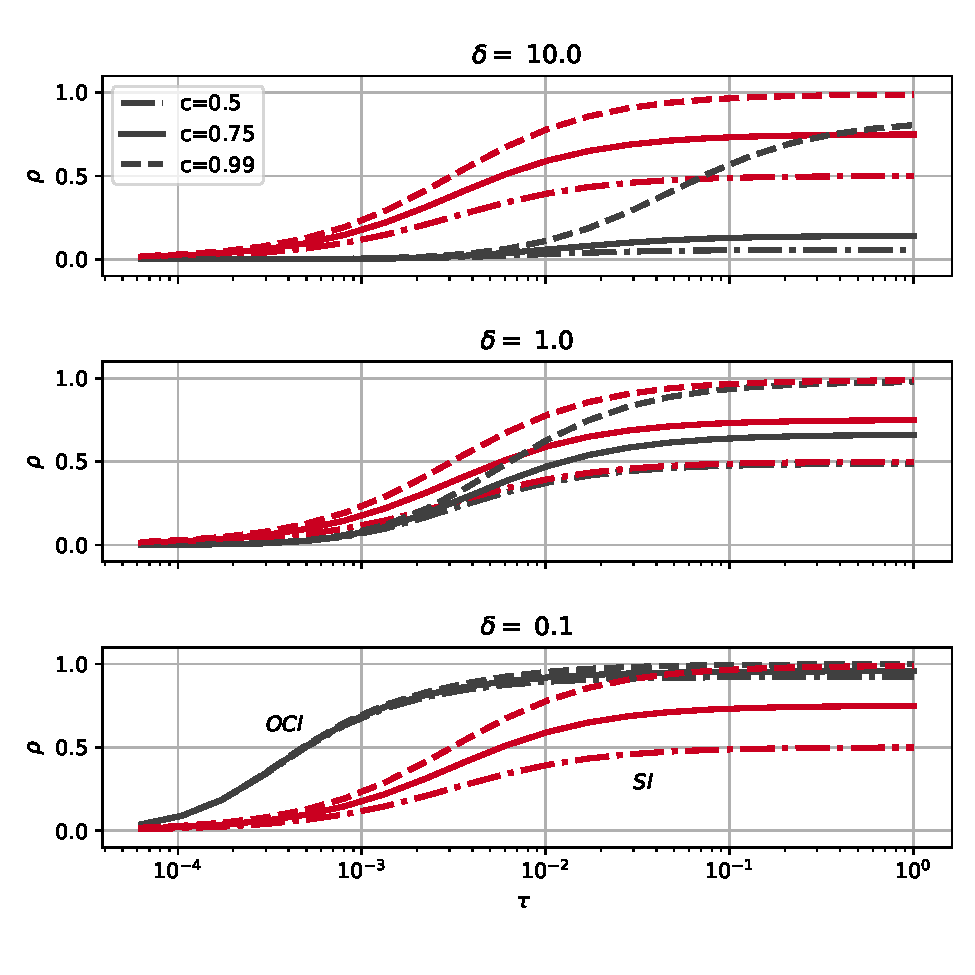
\includegraphics[width=\textwidth]{manuscript2/man2_figs/spec_rad_over_dt.pdf}
    \caption{Spectral radius of OCI (black) and SI (red) over choices of mean free path ($\delta$), time step ($\Delta t$), and scattering ratio ($c$).}
    \label{fig:specrad_fa}
\end{figure}

%Fourier analisys shown in Figure \ref{fig:specrad_fa} correctly predict the empirically measured spectral radii from both OCI and SI solvers when running a large slab wall problem with length \SI{100}{\centi\meter}, vacuum boundary conditions, a convergence tolerance of \num{1e-9}, a random (uniform [0,1]) initial guess for the angular flux, and no material source.
%The random initial guess excites all error modes and eases the computing of error between subsequent iterations.

%Generally, the  eigenvalue spectrum for OCI is more intricate than that of SI.
%SI's are almost entirely positive-real with small positive and negative imaginary values (reflected over the real axis due to complex conjugates).

Fourier analysis results also show that, depending on the location in parameter space, the dominant eigenvalue ($|\lambda_{max}|$) can have large imaginary components, with positive or negative real components and complex conjugate reflections over the real axis.
Complex dominant eigenvalues leading to oscillatory convergence patterns have previously been identified in spatial domain decomposition algorithms where $\rho=1$ when $\delta \rightarrow 0$ \cite{compeig2019ani}. 

%We are unaware if this more nuanced eigenvalue spectrum impacts any behavior of OCI but generally large magnitude imaginary values may indicate some oscillatory behavior.
Deterministic solvers are commonly verified against predictions of $\rho$ from Fourier analysis.
We attempted to do the same by running a problem with length \SI{100}{\centi\meter}, vacuum boundary conditions, a convergence tolerance of \num{1e-13}, $\Sigma=$ \SI{2.5}{\per\centi\meter}, $\Delta x=$ \SI{0.10}{\centi\meter}, $c=$ \num{0.9}, $\Delta t=$\SI{0.10}{\s}, $v=$ \SI{4.0}{\meter\per\s} ($\delta =$ \num{0.25}, $\tau=$ \num{1.0}), a random (uniform [0,1]) initial guess for the angular flux, and no material source in S$_8$.
The random initial guess excites all error modes and provides an anaclitic solution ($\Psi^{\text{converged}} = 0$) to compute iteration errors.
Figure \ref{fig:eigplot} on the left shows the predicted eigenvalues from Fourier analysis and indicates the dominant eigenvalue that contributes to $\rho$ for this particular problem.
In this case, that dominant eigenvalue has considerable real and complex components at $\lambda_{max} =$ \num{0.429} $+$ \num{0.216}$i$ and $\rho=$ \num{0.4831}.
%The plot in the middle of Figure \ref{fig:eigplot} shows the residuals measured from the transport solver when this problem is executed.

Figure~\ref{fig:eigplot} on the right shows $\rho$ predicted from Fourier analysis (flat constant line) as well as $\rho$ measured from the ratio of subsequent residuals as a function of iteration count ($l$).
The empirically estimated value of $\rho$ oscillates around the predicted spectral radius until convergence, with a measured amplitude around \num{0.1}.
The oscillation of the empirically measured spectral radius also seems to grow through iteration count, which may be due to the compounding impact of truncation error and/or machine precision.
So, we cannot rigorously verify our implementation of OCI via Fourier results, because only a mean of the oscillation will match the only-real $\rho$ provided from Fourier results ($|\lambda_{max}|$).
More work is warranted to develop methods that can better capture the empirical behavior of the ratio of subsequent residuals produced from a transport solver and relate them to the complex dominant eigenvalues that may be predicted from Fourier analysis.

%Often deterministic transport solvers compare Fourier predictions of $\rho$ to empirically measured $\rho$ from transport iterations to verify their implementation.


\begin{figure}[htbp]
    \centering
    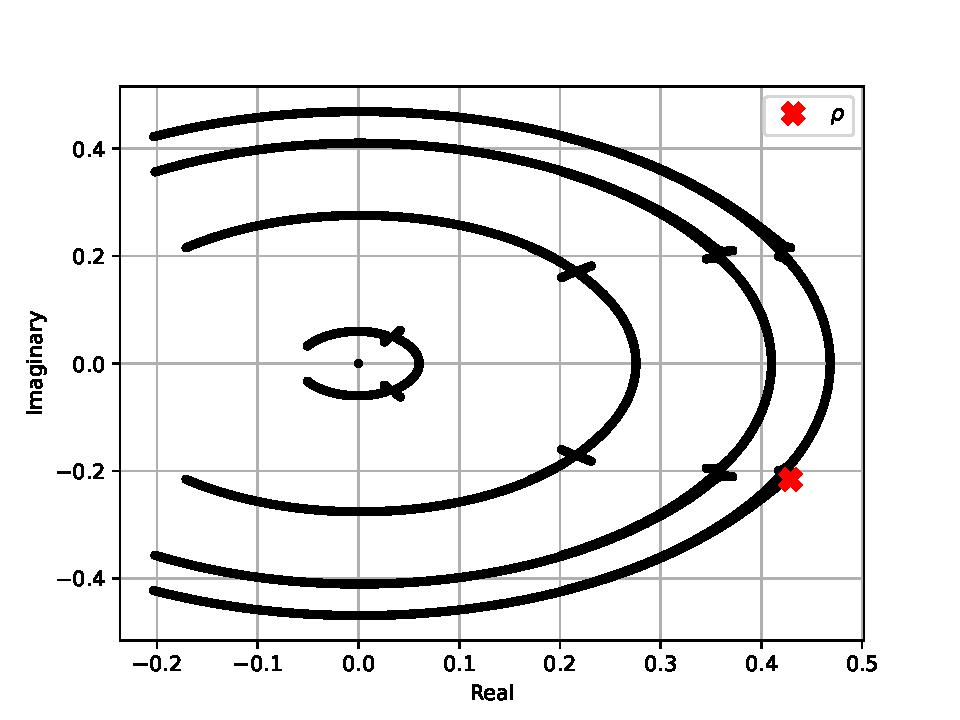
\includegraphics[width=.49\textwidth]{manuscript2/man2_figs/eig_plot.pdf}
    %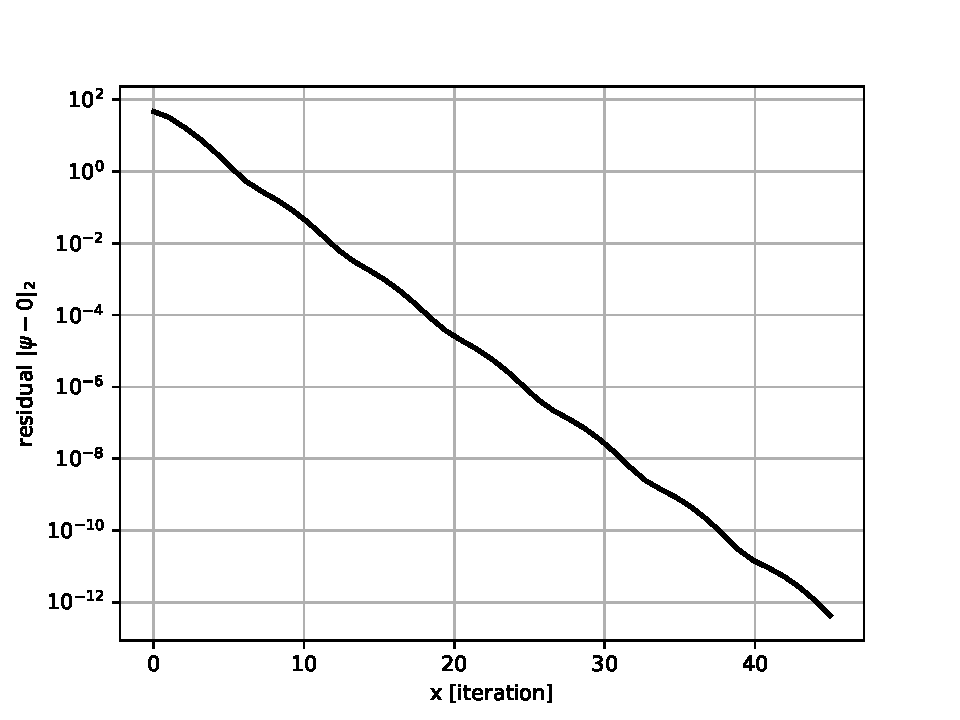
\includegraphics[width=.32\textwidth]{figures/eig_res.pdf} Middle: residual as a function of iteration count from a transport solver,
    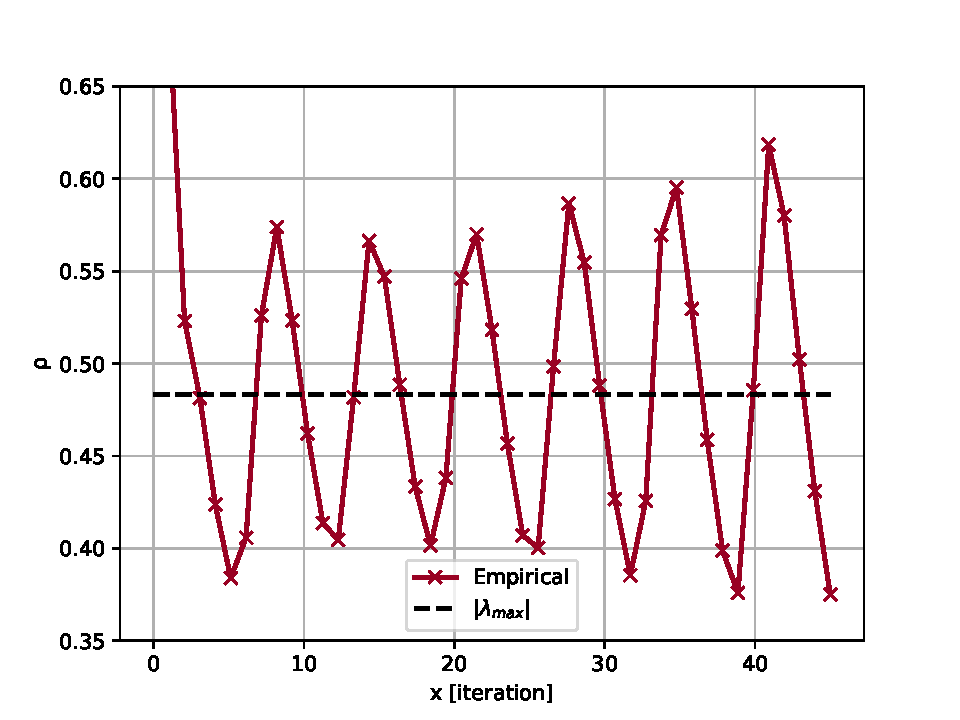
\includegraphics[width=.49\textwidth]{manuscript2/man2_figs/eig_spec_rad.pdf}
    \caption{Eigenvalues in the complex plane of OCI (left), and spectral radius as a function of iteration from the empirical ratio of subsequent residuals and as predicted by Fourier analysis (right).}
    \label{fig:eigplot}
\end{figure}


%The need for a better spectral radius estimate for systems containing complex conjugates eigenvalues has previously been described \cite{variansyah_robust_2021}.
%Theory on complex eigenvalues to an iterative system seems to be sparse in the literature so we leave further exploration of this for future work.



\subsection{Performance on GPUs}

Runtime results were gathered on the Tioga machine at Lawrence Livermore National Laboratory.
Tioga is an early access machine for LLNL's exascale-class El Capitan machine.
On its standard partition, Tioga's nodes have four AMD MI250X GPUs and one AMD EPYC 7A53 CPU.
%Note that a single MI250X itself has two graphics compute dies (GCDs) so one node of Tioga has a total of eight GPUs for MPI purposes; we still report results as if four.
%Tioga also has a partition of AMD MI300A APUs which will be deployed in the exascale-class El Capitan machine.
%Each MI300A is a 24-core CPU on the same die as the GPU.
%The APU architecture of the MI300A is different from previous generations of GPUs as there is little-to-no overhead cost to moving data from the host and device side as device memory is shared between the CPU and GPU components of the APU.
Our methods are currently implemented for a single GPU, so this analysis will be limited to using a single graphics compute die of an MI250X.
We compiled using ROCm version 6.2.1 (includes rocSOLVER and rocBLAS libraries) and used double precision for all values represented.

To analyze performance, we adapt a test problem described by \cite{rosa_cellwise_2013} for a 1D time-dependent, multi-group problem.
Table~\ref{table:rosa_test} describes the material data for this 
two-group problem ($L=$ \SI{100}{\centi\meter}) with vacuum boundary conditions on either side. %Table \ref{table:rosa_test} lists the material data and solver parameters.
The initial condition is $\psi_{t=0} = 0$, and we analyze runtime performance over various choices of $\delta$ and quadrature order at time step sizes of $\Delta t=$ \SI{0.1}{\s} and \SI{10.0}{\s}.
The problem is highly scattering with a maximum scattering ratio of \num{0.99997}.

%Figure blah shows the fourier predictions for 
%When a one group analog limiting senicaro ($c=0.99997$) is used in 

\begin{table}[htb]
  \centering
  \begin{tabular}{@{}c c c c c c@{}} \toprule
    Property & Group 1 & Group 2 & units \\ \midrule
    $\Sigma$ & 1.5454 &  0.45468 & cm$^{-1}$  \\
    $\Sigma_{s,g\rightarrow g}$  & 0.61789 &  0.0072534 & cm$^{-1}$  \\
    $\Sigma_{s,g'\rightarrow g}$  & 0.38211 &  0.92747 & cm$^{-1}$ \\
    $\Sigma_s/\Sigma$ & 0.99997 & 0.86012 & - \\
    $Q$ & 1 & 1 & cm$^{-3}$s$^{-1}$\\
    $v$ & 1 & 0.5 & cm s$^{-1}$ \\
    \bottomrule
  \end{tabular}
  \caption{Test problem material data and simulation parameters.}
  \label{table:rosa_test} 
\end{table}

%Figure \ref{fig:time_desc} shows the number of iterations required to converge using both iterative schemes varying the time step, at various selections of $\Delta x$.
%Again we observe that SI behaves independently of the MFP (and $\Delta x$) so the blue curve is the same on every plot.
%SI does see improved convergence rate with respect to smaller time discretizations which we believe is due to improvements from the scattering ratio.
%OCI improves with \textit{both} larger choices of $\delta$ and smaller times steps---as hypothesized---with smaller time steps being inversely correlated to cellular MFP.
%In fact the rate of improvement of the convergence rate actually actually increases in the thin limit.
%This confirms our hypotheses from observations of the spectral radius, that for smaller time steps OCI converges more rapidly, especially for problems in the thin limit.
%In effect transit works as an acceleration scheme for OCI.

%\begin{figure}[]
%    \centering
%    \includegraphics[width=.75\textwidth]{figures/time_desc.png}
%    \caption{Iteration count of OCI and SI to converge the Rosa problem over various choices of $\Delta t$ and $\rho$ }
%    \label{fig:time_desc}
%\end{figure}

Figure~\ref{fig:runtimes10.0} on the left compares the wall clock runtime of OCI (in black) and SI (in red) over various selections of $\delta$ (controlled via $\Delta x$) with $\Delta t=$ \SI{10.0}{\s}, Figure~\ref{fig:runtimes10.0} on the right shows the speedup of OCI over SI.
In each row, we are increasing quadrature order to increase the overall dimensionality of the system.
Figure \ref{fig:runtimes0.1} shows the same information, but for $\Delta t=$ \SI{0.1}{\s}.
%In a normal compute mode this would be done with the solution from the previous time step.
Runtimes are measured over the convergence loops (see Algorithms \ref{alg:si} and \ref{alg:ocigpu}), so do not include the building and moving the $A_j$ matrices from host to device.
The total cross section used in the $\delta$ scale is the limiting value (the smallest) from group 2 (see Table \ref{table:rosa_test}).

SI's convergence loop runtime increases linearly as cellular optical thickness decreases as there are more cells to solve  in serial.
The number of iterations required to converge the solution is the same but the size of the solution grows.
SI only has $NG$ $4\times4$ systems to solve at any moment so the amount of serial work increases with the number of cells (decreasing $\delta$).
However, as we increase quadrature order the runtime performance of SI actually improves because the solver has more parallelizable degrees of freedom.


\begin{figure}[htbp]
    \centering
    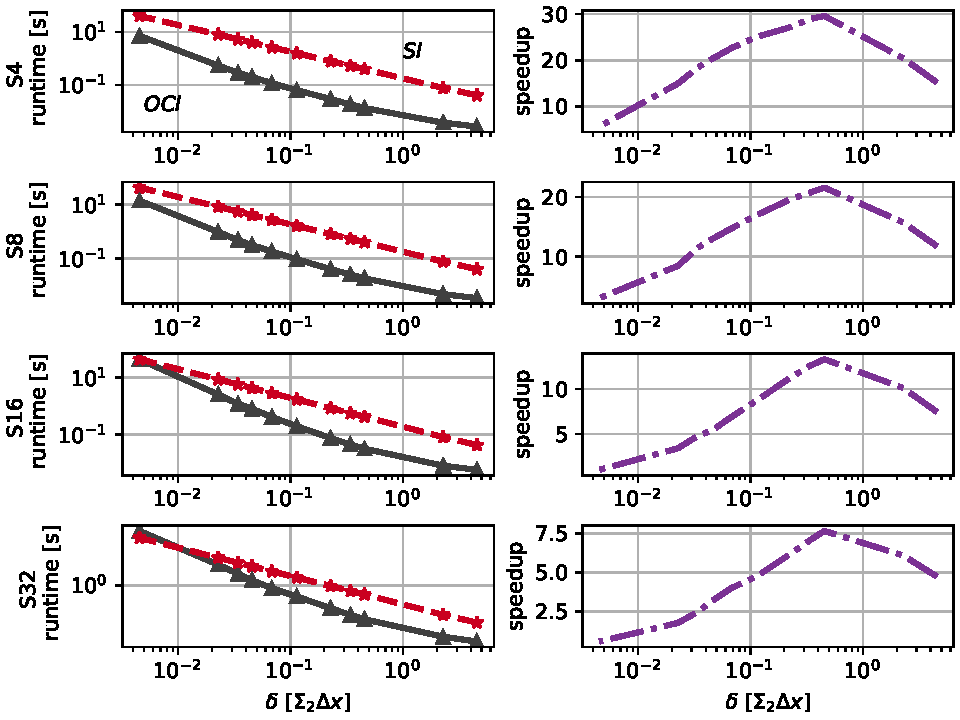
\includegraphics[width=1.0\textwidth]{manuscript2/man2_figs/runtimes_10.0.pdf}
    \caption{Wall-clock runtimes of the convergence loop (left) and 
    speedup of OCI over SI (right) at $\Delta t=$\SI{10.0}{\s} ($\tau=$ \num{2.2734}) as a function of $\delta$ and at various quadrature orders.}
    \label{fig:runtimes10.0}
\end{figure}

\begin{figure}[htbp]
    \centering
    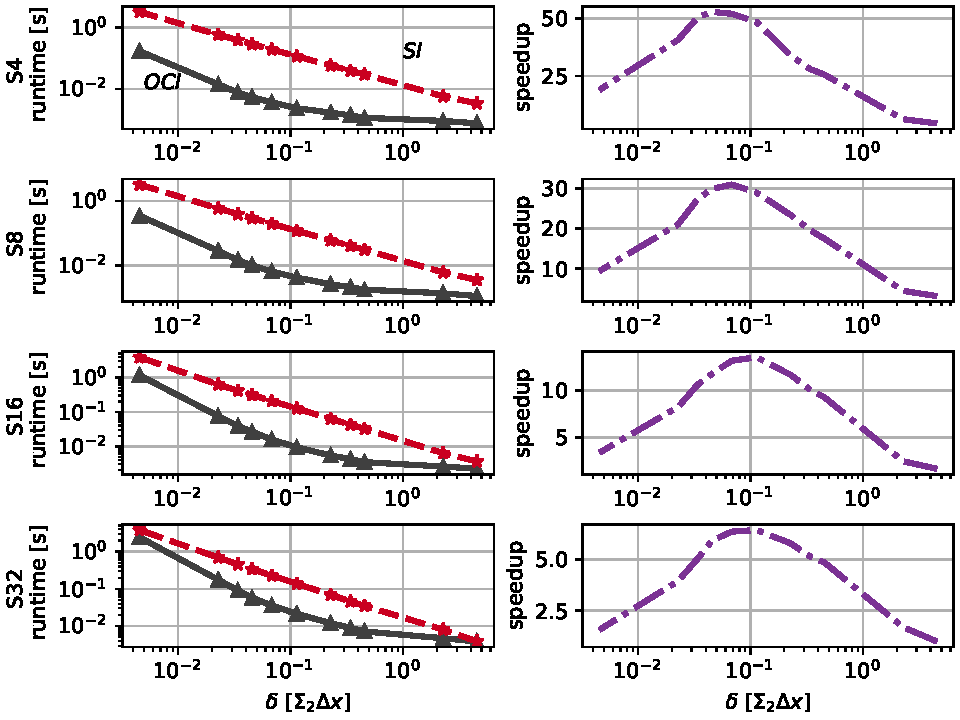
\includegraphics[width=1.0\textwidth]{manuscript2/man2_figs/runtimes_0.1.pdf}
    \caption{Wall-clock runtimes of the convergence loop (left) and 
    speedup of OCI over SI (right) at $\Delta t=$\SI{0.1}{\s} ($\tau=$ \num{0.0227}) as a function of $\delta$ and at various quadrature orders.}
    \label{fig:runtimes0.1}
\end{figure}

For larger time steps, OCI shows less speed-up over SI as it slows for S$_{16}$ and S$_{32}$ quadratures in the thin limit.
The parallelizable degrees of freedom increase with the number of cells (by decreasing $\delta$), but the spectral radius decreases dramatically as cells get thinner.
In the thin limit, OCI requires more iterations to converge the solution, but those iterations can be done faster on the GPU than with SI.
OCI seems to have a ``sweet spot", where the size of the matrices is optimal for the solver, before the spectral radius degrades in the thin limit.
This is observed at around $\delta=4$ for $\Delta t=$ \SI{10}{\s} and $\delta=0.1$ for $\Delta t=$ \SI{0.1}{\s}.
The location of this optimality depends on factors including optimizations at the solver level employed when compiling the vendor-supplied LAPACK libraries \cite{rocsolver}.
The smaller time step increases OCI's relative performance over SI, generally increasing speedup by upwards of 40\% for this highly scattering problem.

%Figure \ref{fig:perf} at right shows the speedup of OCI over SI for that same problem. 
%The previously mentioned "sweet spot" can now be seen as a definite peak around MFP$=0.1$.
%The peak move slightly depending on the number of angles in quadrature.
%In smaller quadrature orders the speedup is the greatest with OCI being about 45 times faster then SI.